\documentclass[a4paper,11pt]{article}
\usepackage{fullpage}
\usepackage{subfigure}
\usepackage{enumitem}
\usepackage{graphicx}
\usepackage{amsmath}
\usepackage{amssymb}
\usepackage{amsthm}

\usepackage{pgf}
\usepackage{float}
\usepackage{multicol}
\usepackage[utf8]{inputenc}
\usepackage[english]{babel}
\usepackage[toc,page]{appendix}
\usepackage{listings}
\usepackage{multidef}
\usepackage{xspace}
\usepackage{algorithmic}
\usepackage[ruled]{algorithm2e}
\usepackage{pdfpages}
\usepackage{standalone}



\newtheoremstyle{break}
{\topsep}{\topsep}%
{\itshape}{}%
{\bfseries}{}%
{\newline}{}%
\theoremstyle{break}
\newtheorem{TLA}{Specification}



\usepackage{tlatex}
\usepackage{color}
\definecolor{boxshade}{gray}{0.9}
\setboolean{shading}{true}

\newtheorem{theorem}{Theorem}[section] 


\lstset{frame=tb,
	aboveskip=3mm,
	belowskip=3mm,
	showstringspaces=false,
	columns=flexible,
	basicstyle={\small\ttfamily},
	numbers=none,
	numberstyle=\tiny\color{gray},
	keywordstyle=\color{blue},
	commentstyle=\color{dkgreen},
	stringstyle=\color{mauve},
	%breaklines=true,
	breakatwhitespace=true,
	tabsize=3
}




\newcommand{\code}[1]{\texttt{#1}}
\setlength{\columnsep}{1cm}
\DeclareMathAlphabet{\mathpzc}{OT1}{pzc}{m}{it}
\newtheorem{definition}{Definition}
\let\cleardoublepage\clearpage
\usepackage{todonotes}
\newcommand{\TJ}[1]{\todo[color=green!50]{\sf \textbf{TJ:} #1}}
\newcommand{\TAP}[1]{\todo[inline,color=red!50]{\sf \textbf{TAP:} #1}}
\newcommand{\MQ}[1]{\todo[inline,color=blue!50!red!10]{\sf \textbf{MQ:} #1}}





\usepackage{multidef}
\usepackage{xspace}
\multidef[prefix=bb]{\mathbb{#1}\xspace}{A-Z,One->1}
\multidef{\textsf{#1}}{Actors,Network,Synchronization,Mailboxes,Communications,mailbox,communication,Mutexes}
\multidef{\textsf{\textit{#1}}\xspace}{send,receive,mutexlock->MutexAsyncLock,mutexunlock->MutexUnlock,mutexwait->MutexWait,mutextest->MutexTest, localcomputation->LocalComputation, asynsend->AsyncSend, asynreceive->AsyncReceive, test->TestAny, wait->WaitAny, localcompute->LocalComputation, request->Requests}


\title{Formal Semantics of the SimGrid Simulator}
\begin{document}
\maketitle

This document tries to formally express the semantic of applications that can be executed in SimGrid, such as MPI applications. The long term goals is to find better reduction algorithms for MPI applications in Mc SimGrid, the model-checker embedded within the SimGrid framework.

\medskip

SimGrid is a simulator of distributed applications. Several user interfaces are proposed, ranging from the classical and realistic MPI formalism, to less realistic simgrid-specific APIs that ease the expression of theoretical distributed algorithms. These user interfaces are built upon a common interface, that is implemented either on top of a performance simulator, or on top of a model-checker exploring exhaustively all possible outcomes from a given initial situation.

\centerline{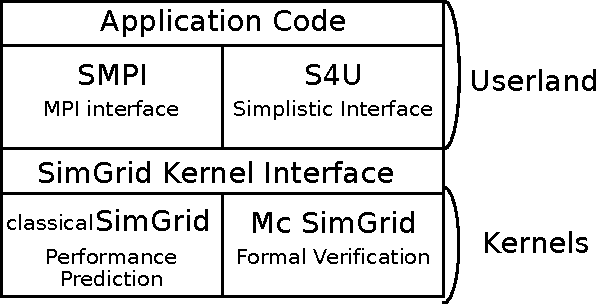
\includegraphics[scale=.6]{Figures/simgrid-architecture.pdf}}

The distributed application is represented in SimGrid as a set of \textbf{actors}, representing  
processes or threads of real applications, or MPI ranks. These actors  interact with each other either through message passing, or with classical synchronization objects (such as mutexes or semaphores), or through executions on CPUs and read/write  operations on disks.

Even if it simulates distributed applications, SimGrid proposes a shared memory model: all actors share the same memory space. To simulate distributed settings, most of the simulated applications simply ensure that they only use variables that are local to each actor, without any program global variables. Enforcing the memory separation at application level allows the kernel to deal with shared-memory and distributed-memory primitives in the same way. It also permits to partially abstract the studied simulated infrastructure: the distributed services that are not relevant to the study can easily be abstracted as centralized components.

From the formal point of view, a major advantage of the SimGrid framework is that all user interfaces are implemented on top of a very small amount of kernel primitives.
In this document, we are interested in formalizing these operations and their inter-dependencies, that will be useful for partial-order reduction methods  in model-checking.

\medskip
This document is organized as follows. Section~\ref{sec:sysdef} formally defines the programming model offered by the SimGrid kernel using TLA+. It specifies the semantic of every offered operation types through their effects on the system. Section~\ref{sec:eventsystem} defines an event system with these operations, exploring the causality, conflict and independence relations between the defined events. Section~\ref{sec:mpi} presents how the MPI semantic is implemented on top of the SimGrid kernel. 
%%%%%%%%%%%%%%%%%%%%%%%%%%%%%%%%%%%%%%%%%%%%%%%%%%%%%%
\newpage 
\section{System State Definition}\label{sec:sysdef}


A distributed system is a tuple $P=\langle \Actors, \Network, \Synchronization \rangle$ in which  $\Actors$ = $\{ A_1, A_2, ... A_n\}$ is a set of $n$ actors. Actors do not have a global shared memory nor a global clock. The execution of an actor $A_i$ consists of an alternate sequence of local states and actions $s_{i,0}\xrightarrow{\text{$a_0$}} s_{i,1} \xrightarrow{\text{$a_1$}}s_{i,2} ... \xrightarrow{\text{$a_{n-1}$}}s_{i,n}$ (firing $a_i$ from local state $s_{i,j}$, the state of actor $A_i$ changes from $s_{i,j}$ to $s_{i,j+1}$).
All the actions in one actor are totally ordered by the causal relation. The subsystem \Network~provides facilities for the \Actors~able exchange messages with each other while subsystem \Synchronization~composed of several mutexes to synchronize actors when they access shared resources. 
\begin{figure}[H]
	\centerline{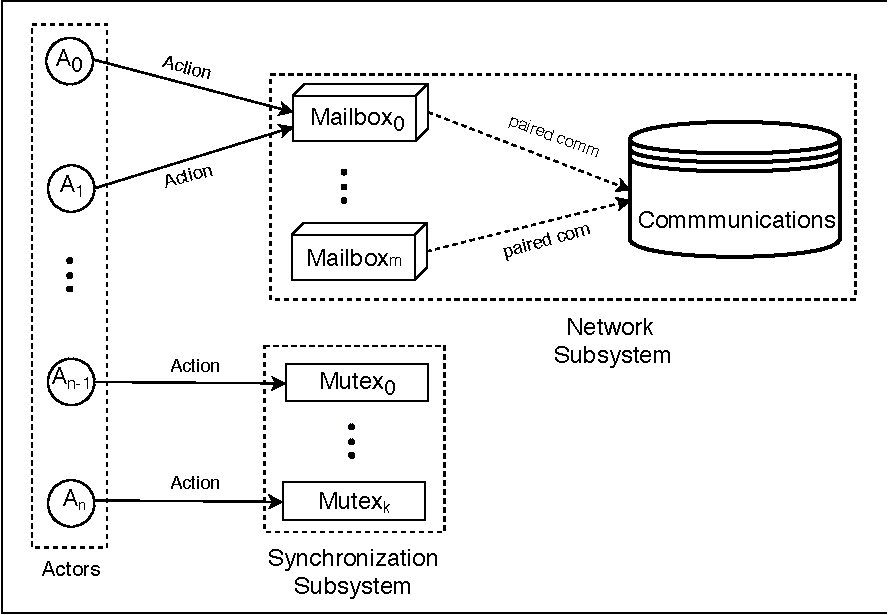
\includegraphics[scale=0.8]{Figures/System.pdf}}
	\caption{Three main elements in the system: \Actors, \Network~and \Synchronization}
\end{figure}



\begin{TLA}[TLA+ specification of functions and variables of the system]
\par\noindent\rule{\textwidth}{0.4pt}
\begin{tlatex}
\input{tlaCodes/declare.txt}
\end{tlatex}
\label{spe.datastructures}
\par\noindent\rule{\textwidth}{0.4pt}
\end{TLA}

We specify $P$ by using a formal specification language called TLA+ \cite{DBLP:conf/sigopsE/LamportMTY02}. Specification \ref{spe.datastructures} is a part of TLA+ specification, presenting variables, data structures for modeling the system. The specification focus on the modeling on how the global states of the system transform by the effect of actions. Actors are identified by actor ids stored in $ActorIds$ set. Each actor has its own memory that can be accessed through variable $memory$ indexed by actor ids. Each instruction in the set $Instr$ correspond an action defined in the next part of specification. The variable $pc$ is an instruction array presenting the current instruction of the actors. Based on the value of the instruction of $pc[aId]$, the correspond action is invoked to execute. Hence, an actor can execute a consequence of actions by changing their instruction in variable $pc$. $Variables$, $Comunications$, $Mutexes$, $MtRequests$ will be used to expressed the state of \Network~and \Synchronization~subsystems. 
 
\subsection{Network Subsystem}
The state of the network subsystem is defined as a pair $\langle \Communications, \Mailboxes \rangle$, where \begin{itemize}[noitemsep]
	
	
\setlength{\itemsep}{3pt}

\item $\Communications$ is a set of individual communications, each of them describing a data exchange  between two actors.  A $\communication$ with the "done" status is formed when a $\send$ communication matches with a $\receive$ communication in a particular mailbox while a communication whose status is "\send" or "\receive" is waiting for the supplement information to create a complete communication (done communication)


\begin{TLA}[TLA+ specification the \Communications]
	\par\noindent\rule{\textwidth}{0.4pt}
	\begin{tlatex}
		\input{tlaCodes/communications.txt}
	\end{tlatex}
	\par\noindent\rule{\textwidth}{0.4pt}
\end{TLA}

\item $\Mailboxes = \{ \mailbox_1, \mailbox_2, ... \mailbox_m \}$ is a set of $m$ mailboxes, each $\mailbox_i$ is an infinite queue storing $\send$ and $\receive$ communications of agents, it is considered as a rendez-vous
where $\send$ and $\receive$ communications meet. For a given mailbox, corresponding communications are stored with a FIFO policy. It means that when a $\send$ communication coming to the mailbox, the oldest $\receive$ is selected to combine with the coming $\send$, producing a ready communication in \Communications~ (the same process for receive communications). Hence, at the same time there are only one kind of pending communications: send or receive communications. 
\begin{figure}[H]
\centerline{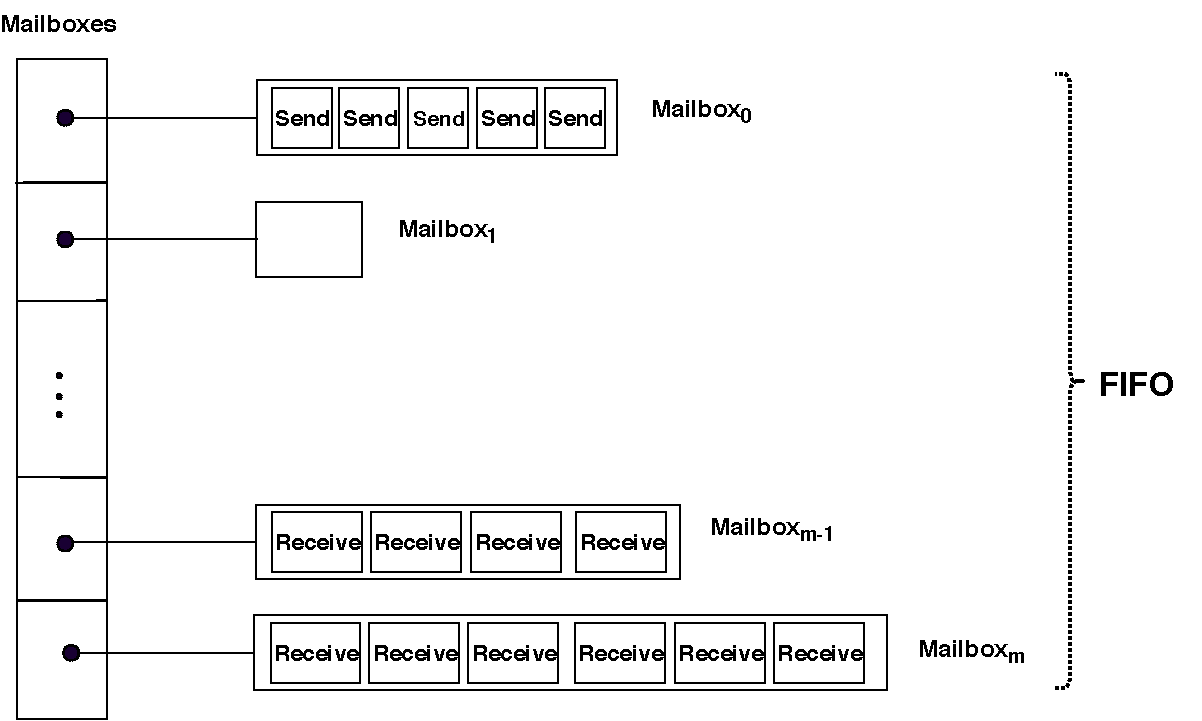
\includegraphics[scale=.55]{Figures/Mailboxes.pdf}}
\caption{\Mailboxes~includes $m$ FIFO mailboxes containing send or receive communications}
\end{figure}


\begin{TLA}[TLA+ specification of the \Mailboxes]
	\par\noindent\rule{\textwidth}{0.4pt}
\begin{tlatex}
\input{tlaCodes/mailboxes.txt}
\end{tlatex}
\par\noindent\rule{\textwidth}{0.4pt}
\end{TLA}
\end{itemize}
Four action types are defined in \Network~subsystem to support actors communicate with each other. They are \asynsend, \asynreceive, \wait~ and \test. An actors start a communication by firing a \asynsend~or \asynreceive; however, data are really exchanged between two actors after firing \wait~or \test~actions. The specification of the actions in $TLA+$ are as follows:     
\begin{itemize}[noitemsep]
\setlength{\itemsep}{3pt}
\item \asynsend


\begin{TLA}[TLA+ specification \asynsend]
\par\noindent\rule{\textwidth}{0.4pt}
\begin{tlatex}
\input{tlaCodes/send.txt}
\end{tlatex}
\par\noindent\rule{\textwidth}{0.4pt}
\end{TLA}

 An actor drops an asynchronous \send~communication to a particular mailbox by firing an \asynsend~action. If there are pending \receive~communications in the mailbox, the \send~communication will be matched with the oldest receive to form a \communication~with "done" status in the \Communications, and the data is copied from the source to the destination. In the other hand, there is no pending receive in the mailbox, a \communication~whose status is "send" is created the mailbox. 
\item \asynreceive


\begin{TLA}[TLA+ specification of \asynreceive]
	\par\noindent\rule{\textwidth}{0.4pt}

\begin{tlatex}
	\input{tlaCodes/receive.txt}
\end{tlatex}
\par\noindent\rule{\textwidth}{0.4pt}
\end{TLA}
Actors use \asynreceive~ to post an asynchronous receive communication on a mailbox; the way a receive communication processed is the same as a send communication treated. The receive communication is combined with a matching send to form a done communication in \Communications. Otherwise, if there is no pending send, a communication that lacks the sender's information is created in the mailbox. 
\item \test

\begin{TLA}[TLA+ specification of \test]
\par\noindent\rule{\textwidth}{0.4pt}
\begin{tlatex}
\input{tlaCodes/test.txt}
\end{tlatex}
\par\noindent\rule{\textwidth}{0.4pt} 
\end{TLA}
 A \test~tests a set of communications, returning either true or false depending on the status of the communications. If at least one communication in the set has a "done" status, \test~action returns true, otherwise false is given. 
\item \wait
\begin{TLA}[TLA+ specification of \wait]
\par\noindent\rule{\textwidth}{0.4pt}
\begin{tlatex}
	\input{tlaCodes/wait.txt}
\end{tlatex}
\par\noindent\rule{\textwidth}{0.4pt} 
\end{TLA}
A \wait~action wait a set of communications, if at least one communication in the set has a "ready" status it become enabled. So, it can blocks it's actor in the case there is no ready communication in the set. 
\end{itemize}

\subsection{Synchronization subsystem}

The state of the \Synchronization~ subsystem is defined by \Mutexes.  $\Mutexes$ = $\{m_1, m_2 ... m_k \}$ is a set of k asynchronous mutexes. The $\Mutexes$ are used to synchronize the actors. An actor $A_i$ declares it's interest on a mutex $m_j$ by executing the action $\mutexlock(A_i,m_j)$~  while the mutex remembers that interest by adding the id of the actor to it's waiting queue. This queue also follows a FIFO policy. We say that a mutex $m$ is $busy$ if there is at least one actor in it's waiting queue, otherwise it is $free$. The state of the $\Mutexes$ can be indicated by state of all the mutexes, more formally the state of $\Mutexes$ = $\{state_1, state_2 ... state_k \}$ where $state_i$ $\in$ \{"free", "busy" \}. 


\begin{figure}[H]
	\centerline{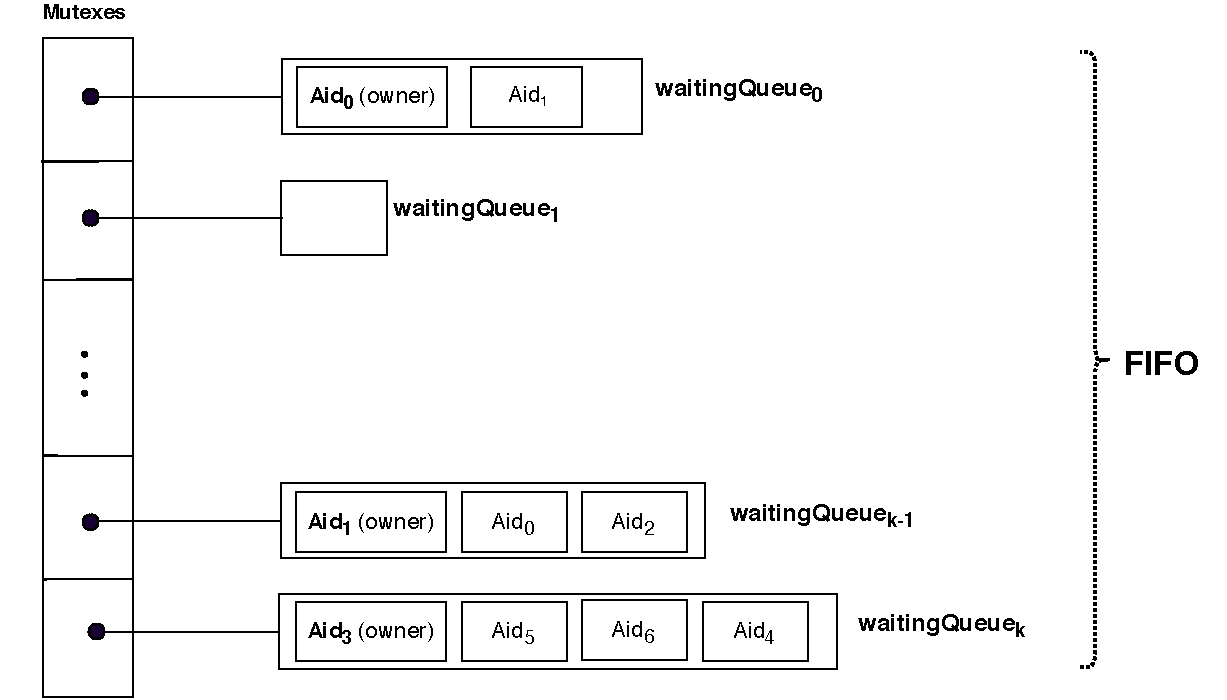
\includegraphics[scale=.55]{Figures/Mutexes.pdf}}
	\caption{ Each mutex uses a waiting queue consisting of actor identifiers}
\end{figure}

In this model mutexes are asynchronous, similar to communication, in the sense that communicationing a mutex is not blocking.  In the synchronization subsystem, there are four actions  allowing actors to interact with the \Mutexes, namely \mutexlock, \mutexunlock, \mutexwait~and \mutextest. They are described formally by $TLA+$ as follows:
 
 \begin{itemize}[noitemsep]
\setlength{\itemsep}{3pt}
\item \mutexlock  
\begin{TLA}[TLA+ specification of \mutexlock]
\par\noindent\rule{\textwidth}{0.4pt}
\begin{tlatex}
\input{tlaCodes/mlock.txt}
\end{tlatex}
\par\noindent\rule{\textwidth}{0.4pt} 
\end{TLA}
$\mutexlock(A_i,m_j)$~is executed by an actor $A_i$ when the actor wants to acquire a mutex $m_j$. After firing \mutexlock, the id $i$ of the actor will be added to the tail of the mutex's queue. Hence, if the mutex is free, the actor is the first in the mutex's waiting queue, and it becomes the $owne$ of the mutex, otherwise it is a $waiting$ actor. However, unlike classical mutexes, when an actor is waiting for a mutex, it is not blocked, and to identify which mutexes it has asked for, the mutex's id $j$ is added to it's \request~set.\\ 
\item \mutexunlock  
\begin{TLA}[TLA+ specification of \mutexunlock]
\par\noindent\rule{\textwidth}{0.4pt}
\begin{tlatex}
\input{tlaCodes/munlock.txt}
\end{tlatex}
\par\noindent\rule{\textwidth}{0.4pt} 
\end{TLA}
 \mutexunlock~ is used to remove an interest on a mutex by an actor. Either the actor is the owner or not, this command can be fired by the mutex, deleting the id of the actor from the mutex's queue and removing the mutex's id from actor's request set.\\
 \item \mutextest

\begin{TLA}[TLA+ specification of \mutextest]
\par\noindent\rule{\textwidth}{0.4pt}

\begin{tlatex}
\input{tlaCodes/mtest.txt}
\end{tlatex}
\par\noindent\rule{\textwidth}{0.4pt} 
\end{TLA}

An actor can check if it is the owner of a mutex that he has previously asked for access to (id of the mutex is included in the actor's request set). To realize this, it can use the \mutextest~action, returning true if the id of the actor is the first element of the mutex's waiting queue, otherwise the returned value is false.\\  

\item \mutexwait 
\begin{TLA}[TLA+ specification of \mutexwait]
\par\noindent\rule{\textwidth}{0.4pt}

\begin{tlatex}
\input{tlaCodes/mwait.txt}
\end{tlatex}
\par\noindent\rule{\textwidth}{0.4pt} 
\end{TLA}
While a \mutextest~can be fired by an actor without a condition ensuring the actor is the owner, a \mutexwait~will not return until it's actor owns the mutex passed to it. Hence, a waiting actor can be blocked when trying to execute a \mutexwait action.
 \end{itemize}

\subsection{Summary}
Actor = local state (containing variables and PC) + program (sequence of actions) 

\noindent\centerline{\begin{tabular}{|c||c|c|}\hline
 \textbf{Subsystem}&\Network&\Synchronization\\\hline\hline
 %
 \textbf{Resource}&Mailbox& Mutex\\\hline
 %
 \textbf{Activity}&Communication&Request\\\hline
 %
 &Send=\asynsend+\wait&Lock=\mutexlock+\mutexwait\\
 \textbf{Actions}&Recv=\asynreceive+\wait&\mutexunlock\\
  &\test&\mutextest\\\hline
\end{tabular}}\\\\\\
\TAP{Please review the next paragraph, I'm not confident with this definition of LocalCompute.}
Beside of the mentioned actions, a program in SimGrid can have local computations named \localcompute~actions. Such actions do not intervene with shared objects (\Mailboxes, \Mutexes~and \Communications), and they can be responsible for I/O tasks. it's specification is as follows:
\begin{TLA}[TLA+ specification of \localcompute]
\par\noindent\rule{\textwidth}{0.4pt}

\begin{tlatex}
\input{tlaCodes/local.txt}
\end{tlatex}
\end{TLA}
\par\noindent\rule{\textwidth}{0.4pt} 

\section{Independence theorems}
 Let $enabled(s)$ represent the set of actions enabled at state s. We have the definition of independence as follows:

\begin{definition}[Independence]\label{def:indep} 
	We say that two actions $a_1$  and $a_2$ are \emph{independent} and write $I(a_1, a_2)$ if they satisfy the two following conditions (\cite{DBLP:books/sp/Godefroid96}):
\begin{itemize}
	\item Executing an action does not enable nor disable any action that is independent with it.
	\begin{equation}\label{eqEnabledness}
	\forall s \in S: a_1 \in enabled(s) \wedge s\xrightarrow{\text{$a_1$}} s' \implies (a_2 \in enabled(s) \Leftrightarrow a_2 \in enabled(s')).
	\end{equation}
	
	\item The execution order of independent actions does not change their overall result.
	\begin{equation}\label{eqCommute}
	\forall s \in S: a_1, a_2 \in enabled(s) \implies (\exists s', s'' \in S:  
	s\xrightarrow{a_1\cdot a_2} s' \wedge s\xrightarrow{a_2\cdot a_1} s'' \implies s' = s'')
	\end{equation}
\end{itemize}
\end{definition}


\begin{definition}[Dependence]
We say that actions $a_1$ and $a_2$ are \emph{dependent} and write $D(a_1, a_2)$ if they are not independent.
\begin{equation}\label{eqDependence}
D(a_1, a_2) = \neg I(a_1, a_2) \end{equation}
\end{definition}

In the following, we prove several independence theorems, specifying classes of actions that are always independent in our system. Here, we only give a sketch of the proof of the theorems while the full proof (based on the TLA$^+$ of actions) is deferred to Appendix X.

\begin{theorem}\label{th:differingMailbox}
Any two communication actions concerning different mailboxes and performed by different actors are independent, be them \asynsend~actions or \asynreceive~actions.
\end{theorem}
\begin{tla}
\forall a1, a2 \in ActorsIds, mb1, mb2 \in MailboxesIds:
mb1 /= mb2 /\ a1 /= a2 =>
		/\ I(AsyncSend(a1, mb1, _, _), AsyncSend(a2, mb2, _, _))
		/\ I(AsyncReceive(a1, mb1, _, _),AsyncReceive(a2, mb2, _, _))
		/\ I(AsyncSend(a1, mb1, _, _), AsyncReceive(a2, mb2, _, _))
\end{tla}
\begin{tlatex}
 \@x{ \forall\, a1 ,\, a2 \.{\in} ActorsIds ,\, mb1 ,\, mb2 \.{\in}
 MailboxesIds \.{:}}%
\@x{ mb1 \.{\neq} mb2 \.{\land} a1 \.{\neq} a2 \.{\implies}}%
 \@x{\@s{75.28} \.{\land} I ( AsyncSend ( a1 ,\, mb1 ,\, \_ ,\, \_ ) ,\,
 AsyncSend ( a2 ,\, mb2 ,\, \_ ,\, \_ ) )}%
 \@x{\@s{75.28} \.{\land} I ( AsyncReceive ( a1 ,\, mb1 ,\, \_ ,\, \_ ) ,\,
 AsyncReceive ( a2 ,\, mb2 ,\, \_ ,\, \_ ) )}%
 \@x{\@s{75.28} \.{\land} I ( AsyncSend ( a1 ,\, mb1 ,\, \_ ,\, \_ ) ,\,
 AsyncReceive ( a2 ,\, mb2 ,\, \_ ,\, \_ ) )}%
\end{tlatex}

\begin{proof}
Since the actions concern different mailboxes, they change the state of different mailboxes. So, changing their execution orders get the same overall state. Besides, an \asynsend~can neither disable nor enable other \asynsend. 
\end{proof}

\begin{theorem}
An \asynsend~action and an \asynreceive~action are independent if they are performed by different actors.
\end{theorem}

\begin{tla}
	
\forall a1, a2 \in ActorsIds: a1 /= a2 
		=> I(AsyncSend(a1, _, _, _), AsyncReceive(a2, _, _, _))
\end{tla}
\begin{tlatex}
\@x{ \forall\, a1 ,\, a2 \.{\in} ActorsIds \.{:} a1 \.{\neq} a2}%
 \@x{\@s{42.52} \.{\implies} I ( AsyncSend ( a1 ,\, \_ ,\, \_ ,\, \_ ) ,\,
 AsyncReceive ( a2 ,\, \_ ,\, \_ ,\, \_ ) )}%
\end{tlatex}

\begin{proof}
Let $a_s$ and $a_r$ be respectively be an \asynsend and an \asynreceive actions. If $a_s$ and $a_r$ occur on differing mailboxes, they are independent by Theorem~\ref{th:differingMailbox}.
 
 Let's assume that they occur on the same mailbox. Let's prove that property (\ref{eqEnabledness}) of Definition~\ref{def:indep} holds in all cases. We use the fact that the mailbox contains a FIFO queue which can either be empty, or contain only send actions, or only receive actions.
(i) If the mailbox's queue initially is empty, $a_s$ and $a_r$ will be matched together. 
(ii) If the mailbox contains send actions before $a_s$ and $a_r$ are triggered, $a_r$ will be matched with the first of the pre-existing send actions and $a_s$ will be added to the tail of the queue. 
(iii) Conversely, if the mailbox initially contains receive actions, $a_s$ will be matched with the first of these recv actions, and $a_r$ will be queued.
In all cases, the outcome does not depend on the relative order of $a_s$ and $a_r$, and Def 1.1 is true. 

In addition, since send and receive actions are never disabled once they exist, Def 1.2 is trivially true. We thus conclude that $I(a_s, a_r)$.
\end{proof}

\begin{theorem}
Two \test~actions, or \wait~actions , or a \wait~action and a \test~action  performed by different actors are independent.
\end{theorem}
\begin{tla}
\forall a1, a2 \in ActorsIds: a1 /= a2 => 
	     /\ I(WaitAny(a1, _), WaitAny(a2, _))
	     /\ I(TestAny(a1, _, _), TestAny(a2, _, _))
	     /\ I(WaitAny(a1, _), TestAny(a2, _, _))   
\end{tla}
\begin{tlatex}
\@x{ \forall\, a1 ,\, a2 \.{\in} ActorsIds \.{:} a1 \.{\neq} a2 \.{\implies}}%
 \@x{\@s{30.61} \.{\land} I ( WaitAny ( a1 ,\, \_ ) ,\, WaitAny ( a2 ,\, \_ )
 )}%
 \@x{\@s{30.61} \.{\land} I ( TestAny ( a1 ,\, \_ ,\, \_ ) ,\, TestAny ( a2
 ,\, \_ ,\, \_ ) )}%
 \@x{\@s{30.61} \.{\land} I ( WaitAny ( a1 ,\, \_ ) ,\, TestAny ( a2 ,\, \_
 ,\, \_ ) )}%
\end{tlatex}
\begin{proof}
 Let's start with two \test~actions. Let $t_1$ and $t_2$ be the first \test~and the second \wait~respectively. (i) Assuming that $t_1$ test communication $com_1$ while $t_2$ test communication $com_2$. With any execution orders,  $t_1$ returns a boolean value based on the status of $com_1$ while a boolean result is given by $t_2$ based on $com_2$. (ii) If both actions are related to the same communication, $t_1$ and $t_2$ return a same boolean result, and they do not depend on the order in which they are executed. From the above claims, changing the execution order get the same final state, Def 1.1 is true.  Besides, because two \test~actions can not enable or disable each other, Def 1.2 is true. Hence, we have I($t_1,t_2)$. Similarly, we have the proof for two \wait~actions, and for a \wait~ and a \test. 
\end{proof}

\begin{theorem}
A \wait~action or a \test~action and a \asynsend~action or a \asynreceive~action are independent if they concern different communications and are performed by different actors. 
\end{theorem}
\begin{tla}
\forall a1, a2 \in ActorsIds, comm1, comm2 \in Addresses:
	/\ a1 /= a2
	/\ Memory[a1][comm1] /=   Memory[a1][comm2]
	=>  /\ I( WaitAny(a1, {comm1}), AsyncSend(a2, _, _, comm2)) 
            /\ I( WaitAny(a1, {comm1}), AsyncReceive(a2, _, _, comm2)) 
            /\ I(TestAny(a1, {comm1}, _), AsyncSend(a2, _, _, comm2))
            /\ I( TestAny(a1, {comm1}, _), AsyncReceive(a2, _, _, comm2))             
\end{tla}
\begin{tlatex}
 \@x{ \forall\, a1 ,\, a2 \.{\in} ActorsIds ,\, comm1 ,\, comm2 \.{\in}
 Addresses \.{:}}%
\@x{\@s{7.90} \.{\land} a1 \.{\neq} a2}%
 \@x{\@s{7.90} \.{\land} Memory [ a1 ] [ comm1 ] \.{\neq}\@s{8.2} Memory [ a1
 ] [ comm2 ]}%
 \@x{\@s{7.90} \.{\implies}\@s{4.1} \.{\land} I ( WaitAny ( a1 ,\, \{ comm1 \}
 ) ,\, AsyncSend ( a2 ,\, \_ ,\, \_ ,\, comm2 ) )}%
 \@x{\@s{41.81} \.{\land} I ( WaitAny ( a1 ,\, \{ comm1 \} ) ,\, AsyncReceive
 ( a2 ,\, \_ ,\, \_ ,\, comm2 ) )}%
 \@x{\@s{41.81} \.{\land} I ( TestAny ( a1 ,\, \{ comm1 \} ,\, \_ ) ,\,
 AsyncSend ( a2 ,\, \_ ,\, \_ ,\, comm2 ) )}%
 \@x{\@s{41.81} \.{\land} I ( TestAny ( a1 ,\, \{ comm1 \} ,\, \_ ) ,\,
 AsyncReceive ( a2 ,\, \_ ,\, \_ ,\, comm2 ) )}%
\end{tlatex}

\begin{proof}
Let's start with a \wait~and an \asynsend~. (i) If they concern different mailboxes, they are trivially independent since there is not shared states between mailboxes and one can not enable or disable other. (ii) Assuming they concern the same mailbox. In the first order we execute the \wait~before \asynsend, program counter of the actor executing \wait is changed. After that a send request posted to the mailbox. Depending on the state of the mailbox (empty or not), the send request can be matched with a pending receive request, or it will be queued into the mailbox. In the reverse execution order, we get the same outcome, the send request is treated similarly, and the program counter changes. It means that the final outcome is not effected by the execution orders. Concerning the Def 1.2, it is true since both actions can not enable or disable other. Hence, they are independent. \\
The proof for a \wait~ and an \asynreceive, a \test and an \asynsend, or a \test~and an \asynreceive~ are similar. 
 
\end{proof}

\begin{theorem}
\label{theorem6}
Two \mutexlock~actions are independent if they concern different mutexes and are performed by different actors.
\end{theorem}
\begin{tla}
\forall a1, a2 \in ActorsIds, mt1, mt2 \in MutexesIds:mt1 /= mt2 /\ a1 /= a2
	=>	I(MutexAsyncLock(a1, mt1, _), MutexAsyncLock(a2, mt2, _))
\end{tla}
\begin{tlatex}
 \@x{ \forall\, a1 ,\, a2 \.{\in} ActorsIds ,\, mt1 ,\, mt2 \.{\in} MutexesIds
 \.{:} mt1 \.{\neq} mt2 \.{\land} a1 \.{\neq} a2}%
 \@x{ \.{\implies} I ( MutexAsyncLock ( a1 ,\, mt1 ,\, \_ ) ,\, MutexAsyncLock
 ( a2 ,\, mt2 ,\, \_ ) )}%
\end{tlatex}

\begin{proof}
		Since two actions modify the state of different mutexes, the final outcomes are the same. Changing the execution order obtain the same final state. Besides, the Def 1.2 is always true for the pair actions. Hence, we conclude the theorem. 
\end{proof}


\begin{theorem}
	A \mutexlock~action and a \mutexunlock~action are independent if they are performed by different actors.
\end{theorem}
\begin{tla}
\forall a1, a2 \in ActorsIds : a1 /= a2
		=> I(MutexAsyncLock(a1, _, _), MutexUnlock(a2, _))
\end{tla}
\begin{tlatex}
\@x{ \forall\, a1 ,\, a2 \.{\in} ActorsIds \.{:} a1 \.{\neq} a2}%
 \@x{\@s{42.52} \.{\implies} I ( MutexAsyncLock ( a1 ,\, \_ ,\, \_ ) ,\,
 MutexUnlock ( a2 ,\, \_ ) )}%
\end{tlatex}
\begin{proof}
	If they touch different mutexes, they are trivially independent since there is no shared state, and they are enabled and disabled independently. In contrary, they touch the same mutex. We firstly examine the execution order where \mutexlock execute before \mutexunlock. In this case the id of the actor that fire the \mutexlock will be added to the mutex's waiting queue while the id of the mutex is removed from the \request of the actor that fires the \mutexunlock. Similarly, with the reverse order we get the same outcome. In addition, the Def 1.2 is true, sine they can not enable and disable other. 
\end{proof}	
\begin{theorem}
Two \mutexwait~actions, two \mutextest~actions, a \mutexwait~action and a \mutextest~action are independent if they are performed by different actors.
\end{theorem}
\begin{tla}
\forall a1, a2 \in ActorsIds : a1 /= a2 => 
		/\ I(MutexWait(a1, _), MutexWait(a2, _))
		/\ I(MutexWait(a1, _), MutexTest(a2, _, _))
		/\ I(MutexTest(a1, _, _), MutexTest(a2, _, _))	
\end{tla}
\begin{tlatex}
\@x{ \forall\, a1 ,\, a2 \.{\in} ActorsIds \.{:} a1 \.{\neq} a2 \.{\implies}}%
 \@x{\@s{42.52} \.{\land} I ( MutexWait ( a1 ,\, \_ ) ,\, MutexWait ( a2 ,\,
 \_ ) )}%
 \@x{\@s{42.52} \.{\land} I ( MutexWait ( a1 ,\, \_ ) ,\, MutexTest ( a2 ,\,
 \_ ,\, \_ ) )}%
 \@x{\@s{42.52} \.{\land} I ( MutexTest ( a1 ,\, \_ ,\, \_ ) ,\, MutexTest (
 a2 ,\, \_ ,\, \_ ) )}%
\end{tlatex}

\begin{proof}
Regarding to two \mutexwait~actions, they just modify local state of their actors. So, commuting their execution does not change the modification. Besides, one are not enabled or disabled by the execution of other one. Hence, they are independent. The proof for two \mutextest~actions, or a \mutexwait~action and \mutextest~action is similar.
\end{proof}

\begin{theorem}
A \mutexlock~action and a \mutexwait~or \mutextest~action are independent if they are performed by different actors.
\end{theorem}
\begin{tla}
\forall a1, a2 \in ActorsIds: a1 /= a2 =>
		/\ I(MutexAsyncLock(a1, _, _), MutexWait(a2, _))
		/\ I(MutexAsyncLock(a1, _, _), MutexTest(a1, _, _))
\end{tla}
\begin{tlatex}
\@x{ \forall\, a1 ,\, a2 \.{\in} ActorsIds \.{:} a1 \.{\neq} a2 \.{\implies}}%
 \@x{\@s{42.52} \.{\land} I ( MutexAsyncLock ( a1 ,\, \_ ,\, \_ ) ,\,
 MutexWait ( a2 ,\, \_ ) )}%
 \@x{\@s{42.52} \.{\land} I ( MutexAsyncLock ( a1 ,\, \_ ,\, \_ ) ,\,
 MutexTest ( a2 ,\, \_ ,\, \_ ) )}%
\end{tlatex}

\begin{proof}
	Let's prove for a \mutexlock~and a \mutexwait. Not depend on the order of execution, after executing the \mutexlock, the id of the mutex is added to \request of the actor that fires the \mutexlock while the id of the actor is queued to mutex's waiting queue. The state of \mutexwait's actor is changed because the actor's PC chages to next action. From the above mentioned, we obtain the final outcome although we change the execution order. In addition, with these two actions, the Def 1.2 is true since the execution of \mutexlock is not effected by \mutexwait~ and reverse. Hence, we the theorem is proved. For the pair \mutexlock and \mutextest is proved similarly. 
\end{proof}

\begin{theorem}
	A \mutexunlock~action and a \mutexwait~or \mutextest~action are independent if they concern different mutexes and are performed by different actors.
\end{theorem}
\begin{tla}
\forall a1, a2 \in ActorsIds, test_r, req \in Addresses, mt \in MutexesIds:
Memory[a1][req] /= mt /\ a1 /= a2 =>
	    /\ I(MutexUnlock(a1, mt), MutexWait(a2, req))
	    /\ I(MutexUnlock(a1, mt), MutexTest(a2, req, _))
\end{tla}
\begin{tlatex}
 \@x{ \forall\, a1 ,\, a2 \.{\in} ActorsIds ,\, test\_r ,\, req \.{\in}
 Addresses ,\, mt \.{\in} MutexesIds \.{:}}%
\@x{ Memory [ a1 ] [ req ] \.{\neq} mt \.{\land} a1 \.{\neq} a2 \.{\implies}}%
 \@x{\@s{65.44} \.{\land} I ( MutexUnlock ( a1 ,\, mt ) ,\, MutexWait ( a2 ,\,
 req ) )}%
 \@x{\@s{65.44} \.{\land} I ( MutexUnlock ( a1 ,\, mt ) ,\, MutexTest ( a2 ,\,
 req ,\, \_ ) )}%
\end{tlatex}

\begin{proof}
	A \mutexunlock~action and a \mutexwait~action are trivially independent since two actions modify the states of different mutexes and actors, changing the execution order obtain the same final state. Besides, the Def 1.2 is always true for the pair actions. Hence, we conclude the theorem. A \mutexunlock~action and a \mutextest~action can be proved similarly. 
\end{proof}

\begin{theorem}
A synchronization action (\mutexlock, \mutexunlock, \mutextest, \mutexwait) is independent with a communication action (\asynsend, \asynreceive, \test, \wait) if they are performed by different actors. 
\end{theorem}
\begin{tla}
\forall a1, a2 \in ActorsIds: a1 /= a2 =>
		/\ I(MutexAsyncLock(a1, _, _), AsyncSend(a2, _, _, _))
		/\ I(MutexAsyncLock(a1, _, _), AsyncReceive(a2, _, _, _))  
		/\ I(MutexAsyncLock(a1, _, _), WaitAny(a2, _))   
		/\ I(MutexAsyncLock(a1, _, _), TestAny(a2, _, _))   

		/\ I(MutexUnlock(a1, _), AsyncSend(a2, _, _, _))
		/\ I(MutexUnlock(a1, _), AsyncReceive(a2, _, _, _))  
		/\ I(MutexUnlock(a1, _), WaitAny(a2, _))   
		/\ I(MutexUnlock(a1, _), TestAny(a2, _, _))

		/\ I(MutexWait(a1, _), AsyncSend(a2, _, _, _))
		/\ I(MutexWait(a1, _), AsyncReceive(a2, _, _, _))
		/\ I(MutexWait(a1, _), WaitAny(a2, _))
		/\ I(MutexWait(a1, _), TestAny(a2, _, _))

		/\ I(MutexTest(a1, _, _), AsyncSend(a2, _, _, _))
		/\ I(MutexTest(a1, _, _), AsyncReceive(a2, _, _, _))
		/\ I(MutexTest(a1, _, _), WaitAny(a2, _))   
		/\ I(MutexTest(a1, _, _), TestAny(a2, _, _))   
\end{tla}
\begin{tlatex}
\@x{ \forall\, a1 ,\, a2 \.{\in} ActorsIds \.{:} a1 \.{\neq} a2 \.{\implies}}%
 \@x{\@s{42.52} \.{\land} I ( MutexAsyncLock ( a1 ,\, \_ ,\, \_ ) ,\,
 AsyncSend ( a2 ,\, \_ ,\, \_ ,\, \_ ) )}%
 \@x{\@s{42.52} \.{\land} I ( MutexAsyncLock ( a1 ,\, \_ ,\, \_ ) ,\,
 AsyncReceive ( a2 ,\, \_ ,\, \_ ,\, \_ ) )}%
 \@x{\@s{42.52} \.{\land} I ( MutexAsyncLock ( a1 ,\, \_ ,\, \_ ) ,\, WaitAny
 ( a2 ,\, \_ ) )}%
 \@x{\@s{42.52} \.{\land} I ( MutexAsyncLock ( a1 ,\, \_ ,\, \_ ) ,\, TestAny
 ( a2 ,\, \_ ,\, \_ ) )}%
\@pvspace{8.0pt}%
 \@x{\@s{42.52} \.{\land} I ( MutexUnlock ( a1 ,\, \_ ) ,\, AsyncSend ( a2 ,\,
 \_ ,\, \_ ,\, \_ ) )}%
 \@x{\@s{42.52} \.{\land} I ( MutexUnlock ( a1 ,\, \_ ) ,\, AsyncReceive ( a2
 ,\, \_ ,\, \_ ,\, \_ ) )}%
 \@x{\@s{42.52} \.{\land} I ( MutexUnlock ( a1 ,\, \_ ) ,\, WaitAny ( a2 ,\,
 \_ ) )}%
 \@x{\@s{42.52} \.{\land} I ( MutexUnlock ( a1 ,\, \_ ) ,\, TestAny ( a2 ,\,
 \_ ,\, \_ ) )}%
\@pvspace{8.0pt}%
 \@x{\@s{42.52} \.{\land} I ( MutexWait ( a1 ,\, \_ ) ,\, AsyncSend ( a2 ,\,
 \_ ,\, \_ ,\, \_ ) )}%
 \@x{\@s{42.52} \.{\land} I ( MutexWait ( a1 ,\, \_ ) ,\, AsyncReceive ( a2
 ,\, \_ ,\, \_ ,\, \_ ) )}%
 \@x{\@s{42.52} \.{\land} I ( MutexWait ( a1 ,\, \_ ) ,\, WaitAny ( a2 ,\, \_
 ) )}%
 \@x{\@s{42.52} \.{\land} I ( MutexWait ( a1 ,\, \_ ) ,\, TestAny ( a2 ,\, \_
 ,\, \_ ) )}%
\@pvspace{8.0pt}%
 \@x{\@s{42.52} \.{\land} I ( MutexTest ( a1 ,\, \_ ,\, \_ ) ,\, AsyncSend (
 a2 ,\, \_ ,\, \_ ,\, \_ ) )}%
 \@x{\@s{42.52} \.{\land} I ( MutexTest ( a1 ,\, \_ ,\, \_ ) ,\, AsyncReceive
 ( a2 ,\, \_ ,\, \_ ,\, \_ ) )}%
 \@x{\@s{42.52} \.{\land} I ( MutexTest ( a1 ,\, \_ ,\, \_ ) ,\, WaitAny ( a2
 ,\, \_ ) )}%
 \@x{\@s{42.52} \.{\land} I ( MutexTest ( a1 ,\, \_ ,\, \_ ) ,\, TestAny ( a2
 ,\, \_ ,\, \_ ) )}%
\end{tlatex}

\begin{proof}
	We start by proving the independence relation between a \mutexlock~an \asynsend. Similar to Theorem~\ref{theorem6}, two actions modify state of different objects. While the \mutexlock modifies the state of a mutex, the \asynsend~ modifies the state of a mailbox and \Communications. Hence, we get the same final state. Besides, one action can not be disabled or enabled by firing other one. So, they are independent. Similarly, A \mutexlock~ action is independent with a \asynreceive~action, a \test~action or a \wait~action. 
\end{proof}
\begin{theorem}
A $\localcompute$ action is independent with all other actions performed by other actors.
\end{theorem}
\begin{tla}
\forall a1, a2 \in ActorsIds: a1 /= a2 => 
		/\ I(Local(a1), AsyncSend(a2, _, _, _))
		/\ I(Local(a1), AsyncReceive(a2, _, _, _))  
		/\ I(Local(a1), WaitAny(a2, _))   
		/\ I(Local(a1), TestAny(a2, _, _))   
		/\ I(Local(a1), MutexWait(a2, _))
		/\ I(Local(a1), MutexTest(a2, _, _))
		/\ I(Local(a1), MutexUnlock(a2, _))
		/\ I(Local(a1), MutexLock(a2, _))
\end{tla}
\begin{tlatex}
\@x{ \forall\, a1 ,\, a2 \.{\in} ActorsIds \.{:} a1 \.{\neq} a2 \.{\implies}}%
 \@x{\@s{42.52} \.{\land} I ( Local ( a1 ) ,\, AsyncSend ( a2 ,\, \_ ,\, \_
 ,\, \_ ) )}%
 \@x{\@s{42.52} \.{\land} I ( Local ( a1 ) ,\, AsyncReceive ( a2 ,\, \_ ,\, \_
 ,\, \_ ) )}%
\@x{\@s{42.52} \.{\land} I ( Local ( a1 ) ,\, WaitAny ( a2 ,\, \_ ) )}%
\@x{\@s{42.52} \.{\land} I ( Local ( a1 ) ,\, TestAny ( a2 ,\, \_ ,\, \_ ) )}%
\@x{\@s{42.52} \.{\land} I ( Local ( a1 ) ,\, MutexWait ( a2 ,\, \_ ) )}%
 \@x{\@s{42.52} \.{\land} I ( Local ( a1 ) ,\, MutexTest ( a2 ,\, \_ ,\, \_ )
 )}%
\@x{\@s{42.52} \.{\land} I ( Local ( a1 ) ,\, MutexUnlock ( a2 ,\, \_ ) )}%
\@x{\@s{42.52} \.{\land} I ( Local ( a1 ) ,\, MutexLock ( a2 ,\, \_ ) )}%
\end{tlatex}


\begin{proof}
\localcompute is trivially independent with other actions sine they modify disjoint parts of the system, and one do not disable or enable other one. 
\end{proof}

%%%%%%%%%%%%%%%%%%%%%%%%%%%%%%%%%%
\section{SimGrid simulations as an Event System}\label{sec:eventsystem}
This section we present how we build the unfolding~\cite{DBLP:conf/concur/RodriguezSSK15}, a Labelled Prime Event Structure (LES for short) of a concurrent program under an independence relation, for our distributed system P by adapting the method in~\cite{DBLP:journals/corr/abs-1802-03950}. We start by defining happen before relations considered as causality relation in LESs. After that, we recap the definition of LES, and finally all steps for constructing an unfolding are described with a simple example illustrating the steps.

\subsection{Happened-before relation}
\begin{figure}[H]
	\label{fig:cycle_dependency}

		%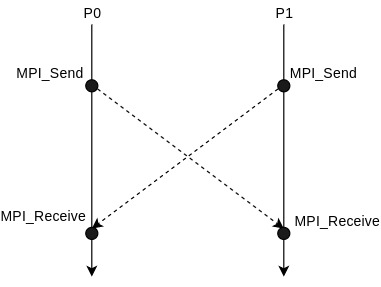
\includegraphics[width=7cm,height=6cm]{example.jpg}
		\centerline{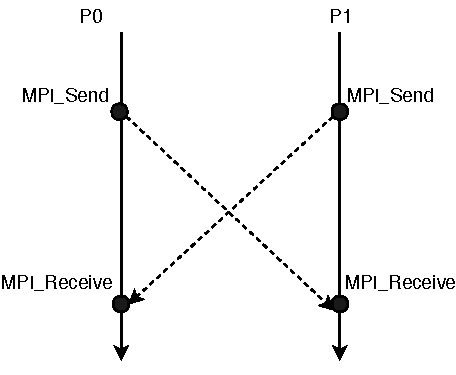
\includegraphics[width=6cm,height=5cm]{Figures/mpiPro.pdf}}
	\caption{A MPI program with a potential deadlock}
\end{figure}
In SimGrid, actions are atomic and actions in the same actor are totally ordered, but actions in the whole system are partially ordered (partial order relation).  Hence, there are different instances (runs) of the system, and the relation between actions are  considered in a given instance. To adapt to the reality, happened-before relation in SimGrid is flexible. Let's look at an example in Figure~\ref{fig:cycle_dependency}. A MPI program including two processes, and process P0 sends a massage to process P1 (doted line). Before receiving  the massage from P0, P1 also sends a massage to P0. At first glance, we may think that there is a deadlock in the program since there is a dependency cycle. However, in practice, depending on the size of the massages exchanged by the processes, the deadlock may appears or not. MPI\_Send and MPI\_Receive are blocking functions in MPI, but they may or may not block. MPI\_Send is ambiguously define, it will not return until the buffer passed to it can be reused. For sending small enough massages, those massages eagerly sent before the calling MPI\_Receive from receiving processes (eager protocol). Hence, MPI\_Sends are not blocked until matching MPI\_Receive have been posted. Actually, if the massages are small, MPI can easily find spaces in internal storage to save them before they are really sent. On the other hand, working with large massages, blocking communications are used, MPI\_Sends must wait for matching MPI\_Receives. Therefor, the scenario in Figure~\ref{fig:cycle_dependency} may or may not has a deadlock. SimGrid covers both cases, users can chose optionally two modes detecting or not deadlocks in the same situation with the above scenario. This conversion can be done easily by switching between two happened\_before definitions.    
  \begin{definition}
  	\label{def:happedBefore1}
  The happened-before relation  denoted by  $\rightarrow $ can be defined based on two relations immediate precede and remotely precede: \begin{itemize}
  	\item Immediate precede (denoted by $ \prec$) :  Two actions e and f in the same actor $A_i$, e $ \prec$ f if the occurrence of e precedes the occurrence of f in the actor $A_i$  
  	\item Remotely precede (denoted by $\leadsto$): Action e is the \asynsend~ or \asynreceive~ action of actor $A_i$, action f is the Wait action of the actor $A_j$,  e $\leadsto$ f if e and f concerns the same communication request.
  	\item The ‘happened before’ is a transitive relation including immediate precede and remotely precede. 
  \end{itemize}\end{definition} 
  
 \begin{figure}[H]
\label{fig:hapend_before}
\subfigure[deadlock]{
		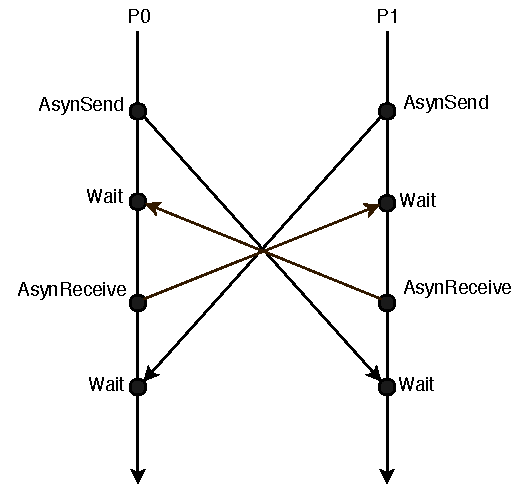
\includegraphics[width=7cm,height=6cm]{Figures/deadlock.pdf}
	}
\hfill
\subfigure[dealock free]{
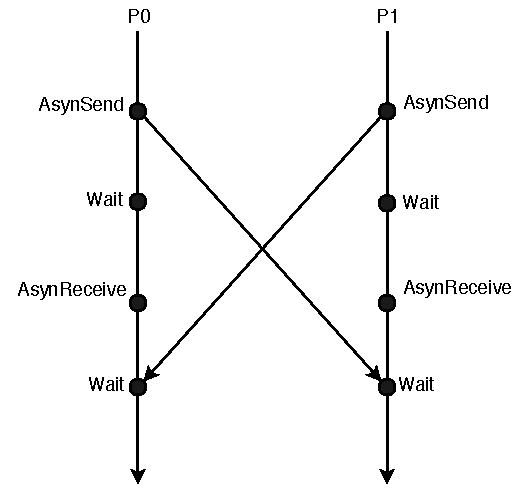
\includegraphics[width=7cm,height=6cm]{Figures/deadlockFree.pdf}
	}
\caption{Happened- before relations between actions}
\end{figure}

The diagram in Figure~\ref{fig:hapend_before}(a) illustrates happened\_before relations (denoted by arrow lines) between actions in the program based on Definition~\ref{def:happedBefore1}. In SimGrid a MPI\_Send is simulated by a \asynsend~ and a \wait~ while a MPI\_Receive comprises a \asynreceive~ and a \wait. Obviously, there is a happened\_before relation cycle in the diagram; the cycle includes the first \wait~ and \asynreceive~ of P0, the first \wait~ and the \asynreceive~ of P1. The existing of cycle leads to a deadlock in the program. In the case we do not want to capture the deadlock, Definiton~\ref{def:happedBefore2} is used.

\begin{definition}
  	\label{def:happedBefore2}
  The happened-before relation  denoted by  $\rightarrow $ can be defined based on two relations immediate precede and remotely precede: \begin{itemize}
  	\item Immediate precede (denoted by $ \prec$) :  Two actions e and f in the same actor $A_i$, e $ \prec$ f if the occurrence of e precedes the occurrence of f in the actor $A_i$  
  	\item Remotely precede (denoted by $\leadsto$): Action e is the \asynsend~action of actor $A_i$, action f is the Wait action of the actor $A_j$,  e $\leadsto$ f if e and f concerns the same communication request.
  \item The ‘happened before’ is a transitive relation including immediate precede and remotely precede.
  \end{itemize}\end{definition} 

Using Definition~\ref{def:happedBefore2} and presenting the happened\_before relation between actions of the program in Figure~\ref{fig:hapend_before}(b), we can see that there are no any cycle, then the program is deadlock-free.

The happened-before relation is not a total order on the actions, two actions may not related by a happened-before relation. In that case, we say that they are concurrent denoted by the symbol $\parallel$. For example, in the above figures, since $\neg$(\asynsend~ of P0 $\leadsto$ \asynsend~ of P1) and $\neg$(\asynsend~ of P0 $ \prec$  \asynsend~ of P1 ) then \asynsend~ of P0 $\parallel$ \asynsend~ of P1.  
\subsection{Event structures}
\textit{Labelled Prime Event Structure (PES for short).} This section recaps the definition of labelled event structures~\cite{DBLP:conf/concur/RodriguezSSK15}

\begin{definition} A labelled event structure on a set label L is a tuple  $\mathpzc{E}$ = $\langle E,<,\#,h \rangle$ where
 \begin{itemize}[noitemsep]
 	\setlength{\itemsep}{2pt}
\item E is a set of events.
\item $<$ is a partial order relation on E, called causality relation.
\item h : E $\rightarrow$ L is a labeling function assigning each event in E to a label in L. 
\item  $\#$ is an irreflexive symmetric relation called conflict relation such that for every event e $\in$ E, the set causes(e) = \{ e' $\in$ E: e'$<e$\} is finite (the set of predecessors of e is finite), and for every events e, f, g $\in$ E, if e \# f and g $<$ f then e \# g.
\end{itemize}
\end{definition}
 Intuitively, the causality relation expresses the happened-before while two events are $conflict$ if they are not in one executions. Each label in L is an action, and if two events neither are $conflict$ nor $causality$ related, they are $concurrent$. An important notion in PESs is $configuration$. A subset of events C of E is a \textit{configuration} if for every event e $\in$ C, $causes(e)$ $\subseteq$ C (all events in causes of e belong to C) and $\forall e, e' \in C, \neg(e \# e')$ (there is no conflict relation in C). We use $Conf(\mathpzc{E})$ to present the set of all configuration in $\mathpzc{E}$.
 
 \section{Unfolding Semantics}

 \textit{Unfolding Semantics (Unfolding for short).} Unfolding Semantics is proposed in~\cite{DBLP:journals/corr/abs-1802-03950} and can describe behavior of a distributed system under independence relations. Indeed, a unfolding is a LES where each maximal configuration corresponds to a Mazurkiewicz trace. In the $unfolding$, each event $e$ is presented by a pair $e$ = $\langle a, H \rangle$ where $a$ is an action in $P$, and $H$ is a history of the event $e$, denoting that action $t$ occurs after the history $H$. For a given configuration $C$, an event $e$ is called maximal event of $C$ if event $e$ is not in the history of other events, more formally $e$ is a maximal event if $\nexists$ $e'$ $\in$ $C$ such that $e < e'$. Let $MaxEvt(C)$ is a set comprised of all maximal events of $C$. Formally, $MaxEvt(C)$ = \{$e$ $\in C $: $\nexists$ $e'$ $\in$ $C$ and $e$ $<$ $e'$ \}. We use $state(C)$ to express the state of application $P$ obtained by executing all actions related to events in $C$ and keep the causality relations in $C$, and $enabled(state(C))$ denotes all actions that enable at $state(C)$
 
  For a given distributed system $P$ and independence relation between actions in $P$, the unfolding of $P$ denoted by $U_P$ = $\langle E,<,\#,h \rangle$, the Algorithm~\ref{Unfolding} illustrates how we build the unfolding of $P$.
  
\begin{algorithm}[H]
	Set all elements $E$, $<$, $\#$, and $h$ are empty\\
	
	\Repeat{No new event added to $E$}{
		\ForEach {subset $E'$ $\in$ E and $E'$ is a configuration} {
			\ForEach {action $a$ $\in$ $enabled(state(E'))$} {
				\If{$D(a, h(e'))$ holds for all $e' \in$ $MaxEvt(E')$}{
					\begin{enumerate}
						\item Add a new event e =  $\langle a , E' \rangle$ to $E$.
						\item Update $<$, $\#$ and $h$ as following:
						\begin{itemize}
							\item[--] set $e' < e$ if  $e' \in E'$.
							\item[--] set $e' \#  e$ if $D(a, h(e')$ and e' $\in$ $E$ $\setminus$ $E$'.
							\item[--] set $h(e) = a$.\\
						\end{itemize}
						   
						
					\end{enumerate}
					
				}
			}
			
		}
	}
	
	
	\caption{Building unfolding\cite{DBLP:journals/corr/abs-1802-03950}}
	\label{Unfolding}
\end{algorithm}

Figure~\ref{fig:unfoldSematics} displays a distributed program $P$ composed of three actors. Actor0 and Actor2 send a $send$ request to the $mailBox1$ while Actor1 posts a $receice$ request on the $mailBox1$. After sending the request, both Actor0 and Actor1 wait the request by firing a \wait~command. Actor1 also declares his interest on the mutex $mutex1$ by executing \mutexlock. The unfolding of the program is described in the right of Figure~\ref{fig:unfoldSematics}. At initial step (denoted by \#) $U_P$ = $\langle \emptyset, \emptyset, \emptyset,\emptyset \rangle$. There is only one configuration C = $\emptyset$ in $Conf(U_p)$. After that events $e_1$ = $\langle \asynsend, \emptyset \rangle$, $e_2$ = $\langle \asynreceive, \emptyset \rangle$ and $e_3$ = $\langle \asynsend, \emptyset \rangle$ are created. We create those events because they have not  precede events, and there is no maximal event in  C to check the dependence condition. We now have four configurations \{$e_1$\}, \{$e_2$\}, \{$e_3$\}, \{$e_1$, $e_2$\}, \{$e_2, e_3$\} and $\emptyset$. For the configuration \{$e_1, e_2$\} we can create event $e_6$ since $pre(e_6)$ = $e_1$ ($e_1$ $\in$ \{$e_1, e_2$\}), the communication is ready, and action $\langle 0, \wait \rangle$ is dependent with $h(e_1)$ and $h(e_2)$. Similarly, we can create events $e_4$, $e_5$, $e_7$, $e_8$, $e_9$ and $e_{10}$. Note that, we have a configuration \{$e_2, e_3, e_8$\}, the maximal events of this configuration are $e_2$ and $e_8$, and $h(e_2)$ $h(e_8)$ are dependently related to action $\langle 0, \wait \rangle$; however, we can not create a new event by combining that configuration with action $\langle 0, \wait \rangle$ because the communication $com$ is not ready for processing in this configuration. The communication $com$ is not ready since there is no pending receive request to march with sending request of Actor0, the receive request already marched with the sending request of Actor2.  We also have the causality relations depicted by arrows, for example $e_1<e_4$, $e_1<e_5$, $e_2<e_6$. Events belong to different configurations are related by conflict relations, for example $e_1 \# e_3$, $e_5 \# e_7$ or $e_3 \# e_9$. In this unfolding, there are two maximal configurations, they are \{$e_1, e_2, e_4, e_5, e_6, e_9 $\}, \{$e_2, e_3, e_7, e_8, e_{10}$\}, and they correspond two Mazurkiewicz traces of the system. 

\begin{figure}[H]
\label{fig:unfoldSematics}

\begin{multicols}{2}
			\centering
			\begin{tabular}{c c}
				\\
				\code{Actor0:}&\code{com = AsynSend(mailBox1) }\\&\code{Wait(com)} \\\\
				\code{Actor1:}&\code{com = AsynReceive(mailBox1)}\\&\code{Wait(com)}\\&\code{MutexAsyncLock(mutex1)} \\\\
				\code{Actor2:}&\code{AsynSend(mailBox1)}
			\end{tabular}

\label{table:ta}

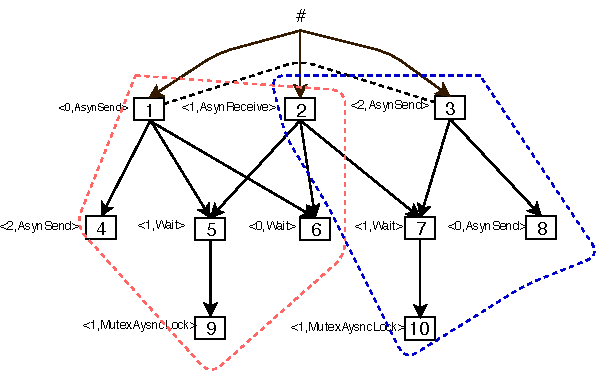
\includegraphics[scale = 0.8]{Figures/unfolding.pdf}

\end{multicols}
\caption{A (toy) program (left), and it's unfolding  semantics (right)}

\end{figure}
\subsection{Determining enabled actions}
In Algorithm \ref{Unfolding}, building unfolding needs compute enabled transitions at state of configurations. Given a configuration $C$, determining enabled action at $state(C)$ can be done trivially by executing all actions related to events in $C$ to obtain the $state(C)$ (executing from initial state of P and preserving causality in $C$), and then checking enabled actions at $state(C)$. However, this solution is very expensive since normally the size of $C$ is large. This section we introduce an efficient method to determining enabled actions at a state of a configuration. 

For an action $a$ in actor $A$, let $pre(a)$ denotes the action is right before $a$ in the actor $A$, and $next(a)$ refers to the next action after $a$. For event $e$ =  $\langle a , C \rangle$, we use $a_e$ to imply the action $a$ that related to event $e$. Given a configuration $C$ and actor $A$, we use $maximalEvent(A,C)$ imply an event $e$ =  $\langle a , C \rangle$ in $C$ such that $\nexists$ an event $e'$ =  $\langle a' , C \rangle$ in $C$ such that $pre(a')$ = $a$, and in this case we say that event $e$ is the maximal event of actor $A$ in $C$. Intuitively, $maximalEvent(A,C)$ is the last occurrence of actor $A$ in the configuration $C$

In the most cases, an action $a$ of actor $A$ is enabled at state of $C$ if it is the next action of the action related to the maximal event of $A$ in $C$. For example, in the Figure \ref{Unfolding}, action $\mutexwait$ is enabled at $state(\{e_2, e_3, e_7\})$ since $maximalEvent(Actor1,C)$ = $e_7$ and $next(\wait)$ = \mutexwait (here \wait~ is the action of event $e_7$). However, in some other cases, the above condition is not enough to ensure an action becomes enabled. For example, action \wait~ of Actor0 is not enabled at $state(\{e_2,e_3,e_7,e_8,e_{10}\})$ although $maximalEvent(Actor0,C)$ = $e_8$ and $next(\asynsend)$ = \wait. The action \wait is not enabled sine the communication $com$ is not ready. Given a \wait~action and assume it wait a $send$ request, to ensure it is enabled at a configuration, there is a available $receive$ can marches with the $send$. We can compare the number of receive request (they must concern the same mailbox with the send request) in the configuration with the number of send request (concern the same mailbox with the send) in the history of event whose action is the send. If the later number is smaller than the former one then the \wait is enabled at the configuration. 


\subsection{UDPOR}

\TAP{Present Unfolding DPOR here, the most important here is how to create new events from current configuration C. From the theory in the paper, for each subset of C, check which actions are enabled at  state($subset_i$(C)). however, how to have the state  state($subset_i$(C)). The worst case is try to run all actions in $subset_i$(C), but it will be very expensive. A smarter solution is based on happended-before relation }

 
\section{MPI Implementation}\label{sec:mpi}

TODO: explain here how MPI is implemented on top of the previously described API
\newpage
\nocite{*}	  	
\bibliographystyle{alpha}
\bibliography{Reference}

%%%%%%%%%%%%%%%%%%%%%%%%%%%%%%5
\newpage
\begin{appendices}

	\begin{theorem}
		An \asynsend~action and an \asynreceive~action are independent.
	\end{theorem}

\begin{proof}
 Suppose both \asynsend and \asynreceive operations are enabled at a state s = $\langle$ \Communications, \Mailboxes, memory, pc, waitingQueue, \request $\rangle$. Let $a_s$ and $a_r$ be respectively the \asynsend and the \asynreceive actions, and let $actor_s$ and $actor_r$ be the actors execute $a_s$ and $a_r$ restrictively. Let's firstly prove that Eq\ref{eqEnabledness} is true.
 
 (i)If they occur on different mailboxes, and suppose that $a_s$ occur on $\mailbox_i$  and $a_r$ occur on $\mailbox_j$. Let's check a situation where $a_s$ is followed by $a_r$. We have $s\xrightarrow{a_s}s_1\xrightarrow{a_r}s_2$, where the state $s_1$ = $\langle \Communications_1$, $\Mailboxes_1$, memory, $pc_1$, $waitingQueue$, $\request$ $\rangle$ and and the state $s_2$ = $\langle$$\Communications_2$, $\Mailboxes_2$, memory, $pc_2$, $waitingQueue$, $\request$ $\rangle$. When firing $a_r$, depending on the state of $\mailbox_i$, the send request can be either added to the LIFO queue of the $\mailbox_i$ if there is no pending request receive, or marched with the first receive request in the queue to form a ready communication $comm$ in \Communications. Hence, in the state $s_1$, \Communications~and \Mailboxes~are replaced by  $\Communications_1$ ( $\Communications_1$ = $\Communications~ \cup$ \{$comm$\} ) ~and $\Mailboxes_1$~respectively. Similarly, the request receive $a_r$ is treated in the same way, it can be queued or marched with a pending send in the $\mailbox_j$. In reverse, executing $a_s$ before $a_r$ obtain the same outcome (state $s_2$).
 
 (ii) If both the request are posted on $\mailbox_i$, we have following cases:
\begin{itemize}
	
\item If the mailbox  is empty, $s\xrightarrow{a_s}s_1$ where the state $s_1$ = $\langle \Communications_1$, $\Mailboxes_1$, memory, $pc_1$, $waitingQueue$, $\request$ $\rangle$ in which $\mailbox_i$ = \{$a_r$\}, the program counter array transform from pc (at sate $s$) to $pc_1$ (at state $s_1$) sine the program counter of $a_s$ changes to the next instruction. After that firing $a_r$ from $s_1$ we have $s_1\xrightarrow{a_r}s_2$ where  $s_2$ = $\langle$$\Communications_2$, $\Mailboxes_2$, memory, $pc_2$, $waitingQueue$, $\request$ $\rangle$. Since there is a pending send request on the mailbox ($a_s$), the request $a_r$ is marched with the send request to create a communication $comm$ in \Communications ($\Communications_1$ = $\Communications~ \cup$ \{$comm$\}). If commuting the execution between $a_s$ and $a_r$, we obtain the same final state (state $s_2$).

\item If the are some pending sends in the mailbox $mailbox_i$, $s\xrightarrow{a_s}s_1$ where the state $s_1$ = $\langle \Communications_1$, $\Mailboxes_1$, memory, $pc_1$, $waitingQueue$, $\request$ $\rangle$. The send request $a_s$ is added to the tail of the mailbox ($\mailbox_i$ = Append ($mailbox_i$, \{$a_s$\}). After that firing $a_r$ at $s_1$, 
$s_1\xrightarrow{a_r}s_2$ where the state $s_2$ = $\langle \Communications_2$, $\Mailboxes_2$, memory, $pc_2$, $waitingQueue$, $\request$ $\rangle$. Because there are some pending send requests in the mailbox, $a_r$ is combined with the first pending send to construct a ready communication in the \Communications. We also reach the final state if apply the reverse order. 

\item If the are some pending receive communications in the mailbox $mailbox_i$, $s\xrightarrow{a_s}s_1$ where the state $s_1$ = $\langle \Communications_1$, $\Mailboxes_1$, memory, $pc_1$, $waitingQueue$, $\request$ $\rangle$. The send request $a_s$ is marched with the first pending receive, creating a communication in \Communications. When a receive request arriving to the mailbox because of executing $a_r$, it will be appended to the tail of the queue ( ($\mailbox_i$ = Append ($mailbox_i$, \{$a_r$\})). If executing $a_r$ before $a_s$ we also obtain the overall state. It means that the final outcome state is not effected by the execution orders. 
\end{itemize}
For the second condition (Def 1.2), based on the condition making $a_s$ enabled \begin{lstlisting}[breaklines=false,  frame=none,	]
  (/\ rdv \in RdV /\ data_r \in Addr/\ comm_r \in Addr /\ pc[aId] \in SendIns)
 \end{lstlisting}
the send action $a_r$ can not be enabled or disabled by the receive action $a_r$, and vice versa $a_r$ is not controlled by $a_s$.

\end{proof}	
	
\begin{theorem}
Two \mutexlock~actions are independent if they concern different mutexes.
\end{theorem}
\begin{proof}
 We will prove that both conditions of the Definition 1 are satisfied. Let's prove that Def 1.1 is true. Suppose both \mutexlock($a_1,m_1$) and \mutexlock($a_2, m_2$) operations are enabled at a state s = $\langle$ Communications, Mailboxes, memory, pc, waitingQueue, Requests $\rangle$. We firstly examine a execution order where \mutexlock($p_1,m_1$) is executed before \mutexlock($p_2,m_2$), and after that, reverse order is checked. We have four cases as follows. 
 \begin{itemize}
 \item If the id of $actor_1$ and $actor_2$ are in included in waitingQueue[m1] and waitingQueue[m2] respectively. This is the simplest situation, and in any order, there is nothing change in the system except the program counter of actor a1 and a2 move to the next instruction. 
  
 \item If the id of $actor_1$ is not in waitingQueue[m1] and the id $actor_2$ is included waitingQueue[m2]. We have $s\xrightarrow{\mutexlock\text{($p_1, m_1$)}}s_1$, where $s_1$ = $\langle$ Communications, Mailboxes, memory, $pc_1$, $waitingQueue_1$, Requests $\rangle$, in which the queue $waitingQueue_1[m_1$] contains the id of $actor_1$, and the program counter of $actor_1$ changes to next instruction. After that, executing \mutexlock($a_2, m_2$) only replaces the program counter of $actor_2$ by the next instruction:  $s_1\xrightarrow{\mutexlock\text{($a_2, m_2$)}}s_2$, where $s_2$ = $\langle$ Communications, Mailboxes, memory, $pc_2$, $waitingQueue_1$, Requests $\rangle$. If we commute the order we will get the final outcome state $s_2$.
 
 \item If the id of $actor_1$ is in waitingQueue[m1], and the id $actor_2$ is not included waitingQueue[m2]. We have $s\xrightarrow{\mutexlock\text{($p_1, m_1$)}}s_1$, where $s_1$ = $\langle$ Communications, Mailboxes, memory, $pc_1$, $waitingQueue$, Requests $\rangle$, everything are unchanged except the program counter of $actor_1$ changes to the next instruction. After that, firing \mutexlock($a_2, m_2$) $s_1\xrightarrow{\mutexlock\text{($a_2, m_2$)}}s_2$, where $s_2$ = $\langle$ Communications, Mailboxes, memory, $pc_2$, $waitingQueue_1$, Requests $\rangle$. This execution adds id of $actor_2$ to  $waitingQueue_1[m_2]$ and $actor_2$'s program counter is moved to the next instruction. The reversed order leads to the same state $s_2$. 
 
    
\item If the id of $actor_1$ and $actor_2$ are not contained in waitingQueue[m1] and waitingQueue[m2] respectively. We have  $s\xrightarrow{\mutexlock\text{($a_1, m_2$)}}s_1 \xrightarrow{\mutexlock\text{($a_2, m_2$)}}s_2$, where $s_1$ = $\langle$ Communications, Mailboxes, memory, $pc_1$, $waitingQueue_1$, Requests $\rangle$ and $s_2$ = $\langle$ Communications, Mailboxes, memory, $pc_2$, $waitingQueue_2$$\rangle$. While $waitingQueue_1[m_1]$ contains $actor_1$, $waitingQueue_2[m_2]$ includes $actor_2$. The array of program counter pc turns to $pc_1$ because the change of program counter of $actor_1$ , and because of the moving that value of $actor_2$ to the next instruction makes $pc_1$ transforms to $pc_2$. For the opposite order where \mutexlock($a_1, m_1)$ goes before \mutexlock($a_2, m_2)$ brings the same overall outcome. 
\end{itemize}
 
Concerning second condition Def 1.2, based on the specification (conditions for enable), it is trivially conclude one can not enable or disable other one. 
 \end{proof}
 
\end{appendices}

\end{document}
